% \documentclass[rnd]{mas_proposal}
\documentclass[thesis]{mas_proposal}

\usepackage[utf8]{inputenc}
\usepackage{amsmath}
\usepackage{amsfonts}
\usepackage{amssymb}
\usepackage{graphicx}

\title{Real-time Learning from Demonstration under Graph-World representation}
\author{Natalia Leonila Quiroga Perez}
\supervisors{Prof. Dr. Paul G. Plöger\\
	Dr. Alex Mitrevski \\}
\date{July 2023}

% \thirdpartylogo{path/to/your/image}

\begin{document}

\maketitle

\pagestyle{plain}

\section{Introduction}

\subsection{Topic of This  Project / Learning from Demonstration }
\begin{itemize}
    \item Provide reasonably detailed description of what you intent to do in your Master Thesis.
    \item You may also discuss the challenges that you have to address.
    \item Reflect on the profile of the reader and PLEAAAASE, tell a story here and refrain from bombarding the readers with details which they may not be able to appreciate.

    Due to the growing acceptance of the use of robots in collaboration with humans in the same environment, Human-Robot Interaction (HRI) is being studied as a successfully emerging area. According to \cite{sheridan2016}, there are four areas of application of HRI; namely, (i) human resources as supervisors in different areas where the tasks are repetitive but robots are still not independent (ii) robots that work in hazardous environments where humans do not have access, and whose movements are usually controlled remotely by an expert, (iii) autonomous robots, such as self-driven cars with humans as passengers, those navigate and plan by sensing their environment, and finally, (iv) robots in a social environment where they interact directly with people, teaching, entertaining, helping children and the elderly.
    
    Specifically, focusing on human-robot social interaction applications, robots used in therapy with children with Autism Spectrum Disorder (ASD) had a positive impact on the patients, as the children had certain preferences for the robot as a therapist instead of an adult; according to \cite{prabha2019}, this is because children with this condition perceive the world differently and robots attract their attention.
    
    In order to encourage patients with autism to learn movements and body language during therapy, the typical procedure is human-human encounters; namely, a selection of imitation games are performed as described in \cite{dautenhahn2004}, where the authors are aware that robots have limited movements, and this method would be difficult to use in a long term therapy, unless the robots increase their behavioural repertoire.
    
    Various procedures can be performed in order to increase the action libraries for the robots. From the naive approach of encoding each and every action, to the more sophisticated approach of using methods to collect demonstrations from humans include different types of motion capture such as kinesthetic guidance \cite{kronander2013}, joystick control \cite{Jiang2013} and kinect camera\cite{assad2020}. Collecting a large number of these demonstrations from non-experts to perform a motion learning procedure is not feasible and tedious for the demonstrator \cite{Chen2022}.
    
    During the study of robots in therapy for ASD, most of the time the main focus are the patients and how the robot affects their reaction, but the therapist also have a reaction to the involvement of robots. In the study by \cite{kulikovskiy2021}, the therapists are the main focus and their preferences are explored, if they do not feel comfortable with the inclusion of new technology and they do not understand how to use it, it may be the case that they go back to traditional methods.
    
    Therapists, as part of the end-user group, should be able to operate the robots with little training and effort. During \cite{kulikovskiy2021}'s experiments with real therapists and the robot Pepper, the main observations were: (i) therapists prefer to teleoperate the robot with Virtual Reality (VR) than to manipulate the robot with a kinesthetic interface; (ii) the use of VR provides a treatment integrity of 83.7\%, which is comparably higher than the 52.9\% of the kinesthetic interface; (iii) therapists found it easier to adapt the therapy to the children's needs with the use of VR; and finally (iv) the workload of task preparation was higher with VR than with kinesthetic interface. 
       
    For instance, the aim is to simplify this process for the demonstrator by making it more user-friendly and faster. The human ability to learn by imitation, and social mirroring \cite{Byrne2005}, inspired Learning from Demonstration (LfD), which has now become an area of extensive research.
    
    In LfD it is necessary to collect examples of optimal sequences of actions or trajectories in order to reproduce similar behaviours \cite{Piot2017}. This can be achieved in two ways; on one hand, Imitation Learning (IL) is a type of supervised learning that consists of learning the mapping between states and actions \cite{Dinyari2020}. On the other hand, Inverse Reinforcement Learning (IRL) has no knowledge of the reward function and tries to learn from the expert's demonstrations \cite{reddy2019}.
    
    The aim of this project is to create a framework that facilitates the process of learning upper limb body movements to extend the action repertoire of robots by capturing skeletal data from non-expert users using an external camera. Subsequently, this library will be stored in order to use the movements in therapy with ASD patients.
    
    The functionality of the framework is divided into two phases, one of which is carried out only once before the non-expert starts the demonstrations; namely, the robot has to carry out a discretization of the environment by performing a space exploration within the limits of the actuators in order to map and recognise the environment and possible obstacles present in its workspace, including its own body structure. The result of this exploration is a set of $n$ graphs, where $n$ is the number of joints of the robot. Each joint graph $i$ has a dependency on the graph $i-1$ of the previous joint. The vertices or nodes represent a reachable point for joint $i$ in the Cartesian space and it stores the position $(x, y, z)$, the joint angles of all previous joints $(1,2,..,i)$ as $(\theta_1, \theta_2,..,\theta_i)$, a state of free or occupied $(0, 1)$, and a list of $k$ joints that can reach the same spatial position in some configuration, it means that this point exists in at least one other graph. 	
 	The edges of all graphs are the Euclidean distance $(d)$ between two nodes, the value of $d$ is constant and determines the quality of the discretisation; namely, the smaller the value of $d$, the higher the quality of the graphs, which means the quality of the movements, the search time and the memory storage also increase; if the value of $d$ is larger, the memory storage and the search time are smaller, but the quality of the path is compromised. Therefore, $d$ has to be carefully tuned to a value that does not compromise either the movements or the time and memory costs.
 	
	The second phase of the framework assumes that the space is partially known to the robot, due to the fact that not all points of the Cartesian space may be explored or there may be more than one robot configuration to reach that point, but enough points have been collected to avoid self-collisions and to detect the static obstacles.  The demonstrations can then be carried out. The skeleton-based data stores the position of the human embodiment. Considering the skeleton upper body part, the joint called "collar" is placed in the center of the body near the chest, this is for the human the base frame $B^H = (0, 0, 0)$, continuously, we can calculate the Spherical coordinates for all the human joints following the equations \ref{eq:radial_distance}, \ref{eq:polar_angle} and \ref{eq:azimuthal_angle}.
	
	\begin{equation}
		 r = \sqrt{x^2 + y^2 + z^2}
	\label{eq:radial_distance}
	\end{equation}
	\begin{equation}
		\theta = \arctan \frac{y}{x}
	\label{eq:polar_angle}
	\end{equation}
	\begin{equation}
		\phi = \arctan \frac{\sqrt{x^2 + y^2}}{z}
	\label{eq:azimuthal_angle}
	\end{equation}

	The transformation gives the polar angle and the azimuthal angle which are the direction of all links. These are then used to calculate the Cartesian coordinates of the robot on its own embodiment following the equations \ref{eq:x_cartesian}, \ref{eq:y_cartesian} and \ref{eq:z_cartesian}. 
	
	\begin{equation}
		x = r \sin \phi \cos \theta
		\label{eq:x_cartesian}
	\end{equation}
	\begin{equation}
		y = r \sin \phi \sin \theta
		\label{eq:y_cartesian}
	\end{equation}
	\begin{equation}
		z = r \cos \phi
		\label{eq:z_cartesian}
	\end{equation}
	Once the desired pose of the robot is found, i.e. the coordinates $(x,y,z)$ of all the joints in Cartesian space, it is possible to search for these coordinates for each joint on each corresponding graph. This would lead to a specific angular configuration of for each captured frame that can be reproduced in the robot under certain constraints.	
\end{itemize}
\subsection{Constraints}
	In this section, the constraints necessary to perform path planning within the discretised representation of the world are introduced.
	\begin{itemize}
		\item IsInside($p$, $j$): The Cartesian points $p$ found for all joints must be inside the workspace of the respective joint $j$. The robot's workspace is not the same workspace for each joint.
		\item IsNode($p$, $g_j$): The Cartesian point $p$ found for all joints is already a node in the graph $g_j$ if the corresponding joint is $j$. If it is not a node and it is inside the workspace, then find the nearest node. If the distance between the candidate node $N_{candidate}$ and the closest node $N_{closest}$ is smaller than the value of the fixed edge $d$ then $N_{closest}$ is added to the path and no new node is created.
		\item CreateNode($p$, $g_j$, $\Theta$, $occupied$): If the distance between $N_{candidate}$ and the closest node $N_{closest}$ is greater than $d$, then the candidate is added to the graph $g_j$ with the corresponding angular configuration of the angles to reach that position. The state "occupied" is initialised with 1 or TRUE.  This new node depends on the previous node where the joint was. For example, there is a direct connection between these two nodes.
		\item MiddleNode($p$, $g_j$, $\Theta$, $occupied$): If the distance between the newly created node and the previous node that the joint occupies is greater than $d$, then $m$ middle nodes are created.  
		
		
	\end{itemize} 
\subsection{Relevance of This Master Thesis}
\begin{itemize}
    \item Who will benefit from the results of this project?
    \item What are the benefits? Quantify the benefits with concrete numbers.
    \item 
    \item 
    \item 
 \end{itemize}

\section{Related Work}

\subsection{Survey of Related Work}
\begin{itemize}
    \item What have other people done to solve the problem?
    \item You should reference and briefly discuss at least the ``top twelve'' related works
\end{itemize}

\subsection{Limitation and Deficits in the State of the Art}
\begin{itemize}
    \item List the deficits that you have discovered in the related work and explain them such that a person who is not deep into the technical details can still understand them.
    For each deficit, provide at least two references
    \item You should reference and briefly discuss at least the ``top twelve'' related works
\end{itemize}

\section{Problem Statement}
\begin{itemize}
    \item Which of the deficits are you going to solve?
    \item What is your intended approach?
    \item How will you compare you approach with existing approaches?
    
     The problem identified during this study is the deficiency in the learning process in humanoid robots of new movements coming from human demonstrators or the lack of a complete system that can perform this learning in an efficient, fast and friendly way for the end-user, in this case the therapist. Without neglecting that there are many important considerations to create a friendly learning systems, it is important to consider the following three questions when intending to use imitation learning as a solution for the above mentioned problem: (i) what to imitate or which is the guiding agent, (ii) how to imitate or what are the tools that allow the desired movement, and (iii) when to perform the imitation to avoid unwanted movements \cite{Billard_2004}; these questions help us define the conditions under which the system can be manipulated. According to \cite{lopes2005developmental}, learning by imitation has three main difficulties: how to collect relevant information to perform a task; how to convert data that is valid for a human into a different body, in this case a robot; and how to select the important parts of the demonstration. These points are developed throughout this work and are explained in detail in the following sections.
    
    This research and development project report presents the process of learning through imitation for robots. To this end, we used QTrobot from LuxAI \cite{qtrobot_safety_manual} and considered both its physical and software features. For the overall learning by imitation process, the first step is identified to be the human action recognition, which can be done through the utilization different methods. For this study, we use depth skeleton motions \cite{Chen_2016}, where the teacher's position is calculated with respect to the camera coordinate system placed on the head of the robot; then, the joint angles describing the full-body are found with the use of an analytic solution to reach the desired positions, and, subsequently, Direct Kinematics (DK) with those angles is performed to calculate the end-effector position \cite{Riley}. Secondly, to remove the effect of frames that contain what we call $noise$, we use filters in order to smooth the joint trajectory signal and we also predict possible collisions by the end-effector in order to avoid damage to the robot and all its parts, which is done by means of the re-estimation of angular positions with Inverse Kinematics (IK). Finally, a control system is proposed in order to improve the precision of the robot's movements.
    
    The content of this work report is organized as follows. Chapter 2 provides the background knowledge required for understanding the field of learning through imitation and provides an overview of the state of the art work existing to date, namely the work in the fields of skeleton recognition, forward and inverse kinematics, collision avoidance and control systems. Chapter 3 describes the problem addressed, and the task of this work as a detailed description of the proposed solution. The performance evaluation of the algorithms given in this approach is presented in chapter 4, as a discussion of the results. Finally, the conclusion of this work and aims of the future research are presented in chapter 5.
\end{itemize}


\section{Project Plan}

\subsection{Work Packages}
\emph{Planning is the replacement of randomness by error.} (Einstein). Very much like you would never start a longer journey without a detailed travel plan, you should not start a project without a carefully though out work plan. A work package is a logical decomposition of a larger piece of work into smaller parts following a ``divide and conquer" strategy. It is very specific to the problem that you are going to address. Refrain from a rather generic decomposition. If your work plan looks similar to those of your school mates, which may address completely different problems then you have not thought carefully enough about how you approach the problem. It is ok to have two generic work packages \emph{Literature Study} and \emph{Project Report}. Discuss your work packages in the ASW seminar.

The bare minimum will include the following packages:
\begin{enumerate}
    \item[WP1] Literature Study
    \item[WP2] ...
    \item[WP3] ...
    \item  ...
    \item[WPy] Evaluation of approach and comparison with similar approaches
    \item[WPz] Project Report
\end{enumerate}

\subsection{Milestones}
Milestones mark the completion of a certain activity or at least a major achievement in an activity. Milestones are also decision points, where you reflect on what you have achieved and what options you have for continuing your work in case you have not achieved what was planned. Above all, milestones have to be measurable. As above, if your milestones are the same as those of your school mates, then you may not have thought carefully enough about how your project shall progress.
\begin{enumerate}
    \item[M1] Literature review completed and best practice identified
    \item[M2] ...
    \item[M3] ...
    \item[M4] Report submission
\end{enumerate}

\subsection{Project Schedule}
Include a Gantt chart here. It doesn't have to be detailed, but it should include the milestones you mentioned above.
Make sure to include the writing of your report throughout the whole project, not just at the end.

\begin{figure}[h!]
    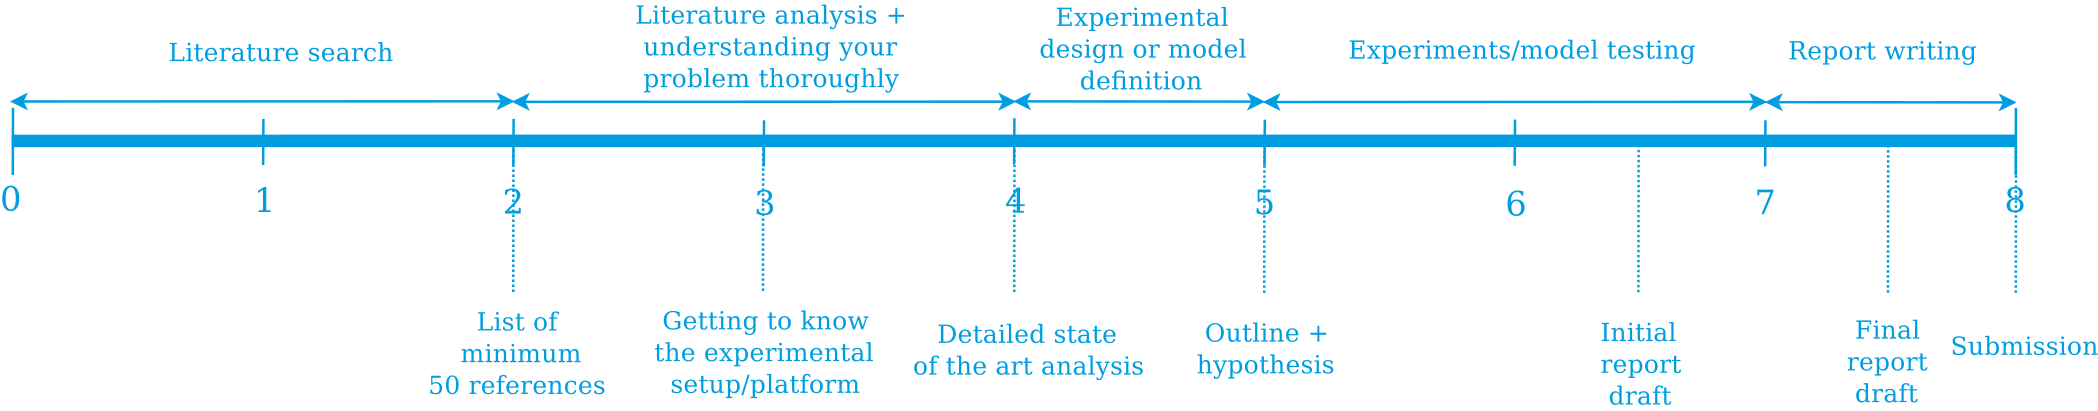
\includegraphics[width=\textwidth]{images/rnd_deliverable_timeline}
    \caption{My figure caption}
    \label{fig:myfigure}
\end{figure}

\subsection{Deliverables}

\subsubsection*{Minimum Viable}
\begin{itemize}
    \item Project results required to get a satisfying or sufficient grade.
\end{itemize}

\subsubsection*{Expected}
\begin{itemize}
    \item Project results required to get a good grade.
\end{itemize}

\subsubsection*{Desired}
\begin{itemize}
    \item Project results required to get an excellent grade.
\end{itemize}

Please note that the final grade will not only depend on the results obtained in your work, but also on how you present the results.

\nocite{*}

\bibliographystyle{plainnat} % Use the plainnat bibliography style
\bibliography{bibliography.bib} % Use the bibliography.bib file as the source of references

\end{document}
